\documentclass[11pt]{article}

\usepackage[margin=1in]{geometry}
\usepackage[T1]{fontenc}
\usepackage[utf8]{inputenc}
\usepackage{lmodern}
\usepackage{microtype}
\usepackage{graphicx}
\usepackage{booktabs}
\usepackage{tabularx}
\usepackage{xcolor}
\usepackage{tcolorbox}
\usepackage[numbers,sort&compress]{natbib}
\usepackage{caption}
\usepackage{float}
\usepackage{hyperref}

\graphicspath{{figures/}}
\hypersetup{colorlinks=true, linkcolor=blue!50!black, citecolor=blue!50!black, urlcolor=blue!50!black}
\captionsetup{font=small, labelfont=bf}

% Open framing decisions for Mark -- delete the boxes once resolved.
\newtcolorbox{framing}{colback=orange!8, colframe=orange!70!black, fonttitle=\bfseries\small,
  title=Framing decision (open), fontupper=\small, left=4pt, right=4pt, top=2pt, bottom=2pt}
\newtcolorbox{notemark}{colback=blue!5, colframe=blue!50!black, fonttitle=\bfseries\small,
  title=Note for Mark (draft only -- remove before release), fontupper=\small, left=4pt, right=4pt,
  top=2pt, bottom=2pt}
\newtcolorbox{pending}{colback=orange!8, colframe=orange!70!black, fonttitle=\bfseries\small,
  title=Pending update, fontupper=\small, left=4pt, right=4pt, top=2pt, bottom=2pt}

\title{Did Generative AI Homogenize Online Writing?\\[4pt]
  \large Evidence from 30 Corpora, 2008--2026}
\author{Mark Nomellini}
\date{Draft v0.2 --- \today}

\begin{document}
\maketitle

\begin{abstract}
We test whether online writing became more homogeneous after the public release of ChatGPT
(2022Q4). We embed the full text of about 1.2 million sampled answers and abstracts from 30 dated
corpora---26 Stack Exchange communities (14 high- and 12 low-cognitive-load) plus Hacker News,
PubMed oncology, arXiv computer science and arXiv mathematics---and test, quarter by quarter, for a
change in trend at 2022Q4. Four findings. (1) Answers became more similar to each other: the similarity trend turns
upward after ChatGPT in 24 of 26 Stack Exchange communities, significantly in 15, and in all 4
external corpora; with a second, independent text encoder the rise holds in expert communities and in
all external corpora, but not in everyday ones. (2) The turn is stronger in high-cognitive-load
communities, where AI saves more effort (11 of 14 versus 4 of 12, and 9 of 14 versus 2 of 12 with
the second encoder; $p\approx0.002$--$0.03$). (3) The change is mainly in \emph{what}
is asked and discussed: the mix of subjects shifts in 24 of 26 communities and answers within the same
subject converge in 18 of 26, but answers to the \emph{same question} converge in only 6. (4) Human
answers do not move towards what a language model would write for the same question. We conclude
that generative AI is associated with a real but specific form of homogenization---a narrowing and
convergence of the questions people bring and the subjects they discuss, strongest in expert
communities---rather than people writing like the model.
\end{abstract}

% ---------------------------------------------------------------------------------------------
\section{Motivation}

Since late 2022 a common complaint has surfaced: \emph{everything online is starting to sound the
same}. As hundreds of millions of people route their writing and their questions through a handful
of large language models, the worry is that the diversity of human expression---and, more
importantly, of \emph{ideas}---collapses towards a shared machine mean.

This matters beyond aesthetics. If the range of answers to a question narrows, so does the pool of
ideas a reader meets. Reference sites and scientific abstracts are the durable memory of a field; if
that record converges, we lose signal about what people actually discovered or argued. There is also
a prior reason to expect an effect: a meta-analysis of human--AI co-creation studies finds a small,
persistent homogenization effect \citep{derooij2026}, and behavioural economics predicts that an
always-available, fluent default answer is exactly the kind of anchor people converge on
\citep{samuelson1988}.

``Did AI homogenize writing?'' is too coarse to test. We split it into four questions, each with its
own test:
\begin{enumerate}
  \item \textbf{Did texts become more similar to each other?} Are two answers from the same quarter more similar after
  ChatGPT than the earlier trend predicts?
  \item \textbf{Where is it stronger?} If AI saves the most effort on demanding questions, the effect
  should be larger in high-cognitive-load communities.
  \item \textbf{What changed?} Texts can become more alike because people discuss a narrower or
  different \emph{set of subjects}, because answers on the \emph{same subject} converge, or because
  answers to the \emph{same question} converge. These have different consequences, and we separate them.
  \item \textbf{Do people write like the model?} Do human answers move towards what a language model
  would write for the same question?
\end{enumerate}

% ---------------------------------------------------------------------------------------------
\section{Data}

All corpora are public, dated to the quarter, and run to 2026Q2, giving 15 quarters of
post-ChatGPT observation against a pre-2022 baseline of 6 to 14 years (Table~\ref{tab:data}).

\textbf{Stack Exchange.} From the June 2026 data dump we use 26 question-and-answer communities with
healthy recent volume: 14 \emph{high-cognitive-load} communities, where questions are technical or
expert (Cross Validated, Philosophy, Economics, Cryptography, Law, History, Computer Science,
Biology, Astronomy, Chemistry, Electrical Engineering, Physics, Software Engineering, English
Language \& Usage), and 12 \emph{low-cognitive-load} ones, about everyday, practical or hobby
subjects (Seasoned Advice, Travel, Bicycles, Gardening, Role-playing Games, Board Games, Personal
Finance, Photography, The Workplace, Home Improvement, Science Fiction \& Fantasy, Arqade). The unit
is a single answer. Each answer is linked to its question and to the question's tags, which the
asker chooses.

\textbf{External corpora.} To check that results are not specific to Stack Exchange's format we add
four corpora from other platforms: Hacker News comments, PubMed oncology abstracts, and arXiv
computer-science and mathematics abstracts. They have no questions or tags, so they are used for the
similarity trend (question 1) and the embedding-topic test (question 3), but not for the
cognitive-load comparison, the tag and same-question tests, or the model anchor, which use the 26
Stack Exchange communities only. Table~\ref{tab:tests} lists the corpora behind each test.

\begin{table}[H]
\centering
\caption{Corpora. Up to 800 texts are sampled per quarter (quarters with fewer than 30 are dropped).}
\label{tab:data}
\small
\begin{tabular}{lrrrl}
\toprule
Group & Corpora & Texts & Sampled & Span \\
\midrule
Stack Exchange, high cognitive load & 14 & 1.80M & 0.54M & 2008Q3--2026Q2 \\
Stack Exchange, low cognitive load  & 12 & 1.08M & 0.50M & 2009Q4--2026Q2 \\
External (HN, PubMed, arXiv CS, arXiv Math) & 4 & 0.21M & 0.13M & 2016Q1--2026Q2 \\
\bottomrule
\end{tabular}
\end{table}

% ---------------------------------------------------------------------------------------------
\section{Method}

\paragraph{Turning texts into vectors.} A sentence encoder---here all-MiniLM-L6-v2
\citep{reimers2019,wang2020minilm}---maps a passage to a vector of 384 numbers such that passages
with similar meaning get vectors pointing in similar directions. The encoder reads at most 128 tokens
(about 90 words) at a time, so to represent a whole answer we clean it of URLs, DOIs, e-mail
addresses and machine strings, split it into sentences, pack the sentences into chunks of at most
120 tokens, embed each chunk, and average the chunk vectors, weighting each by its length.

\begin{notemark}
Draft v0.1 embedded only the first 128 tokens of each text, so it measured how answers \emph{open};
every embedding result in this draft is recomputed on whole texts. Two results changed: the
cognitive-load comparison (Section~\ref{sec:where}) now shows a clear difference, where v0.1 found
none, and same-subject convergence (Section~\ref{sec:what}) is now found on many sites. This note,
and any mention of v0.1, will be removed in the release version.
\end{notemark}

\paragraph{Measuring how alike texts are.} The similarity of two texts is the \emph{cosine
similarity} of their vectors: the cosine of the angle between them, from about 0 for unrelated
texts to 1 for texts with the same meaning (in practice, two random answers from the same community
score about 0.05--0.2). For each corpus and quarter we sample up to 800 texts and take the average
cosine similarity over all pairs of them. A rising average means that texts written in the same
quarter are becoming more similar to one another.

\paragraph{Testing for a change at ChatGPT.} For each corpus we fit a straight trend line to the
quarterly similarity before 2022Q4 and another after it (an \emph{interrupted time series}, or
segmented regression \citep{wagner2002}), with standard errors that allow for correlation between
neighbouring quarters \citep{newey1987}. Our main statistic is the \emph{slope change}: the slope of
the line after ChatGPT minus the slope before, in similarity units per quarter. A positive, significant
slope change means similarity began rising faster (or stopped falling) after ChatGPT;
Figure~\ref{fig:its} shows an example. The same test is applied to every measure below. Because we
test many corpora, we also report how many results survive the Benjamini--Hochberg correction
\citep{benjamini1995}, which limits the expected share of false positives among the results called
significant to 5\%.

\begin{figure}[H]
  \centering
  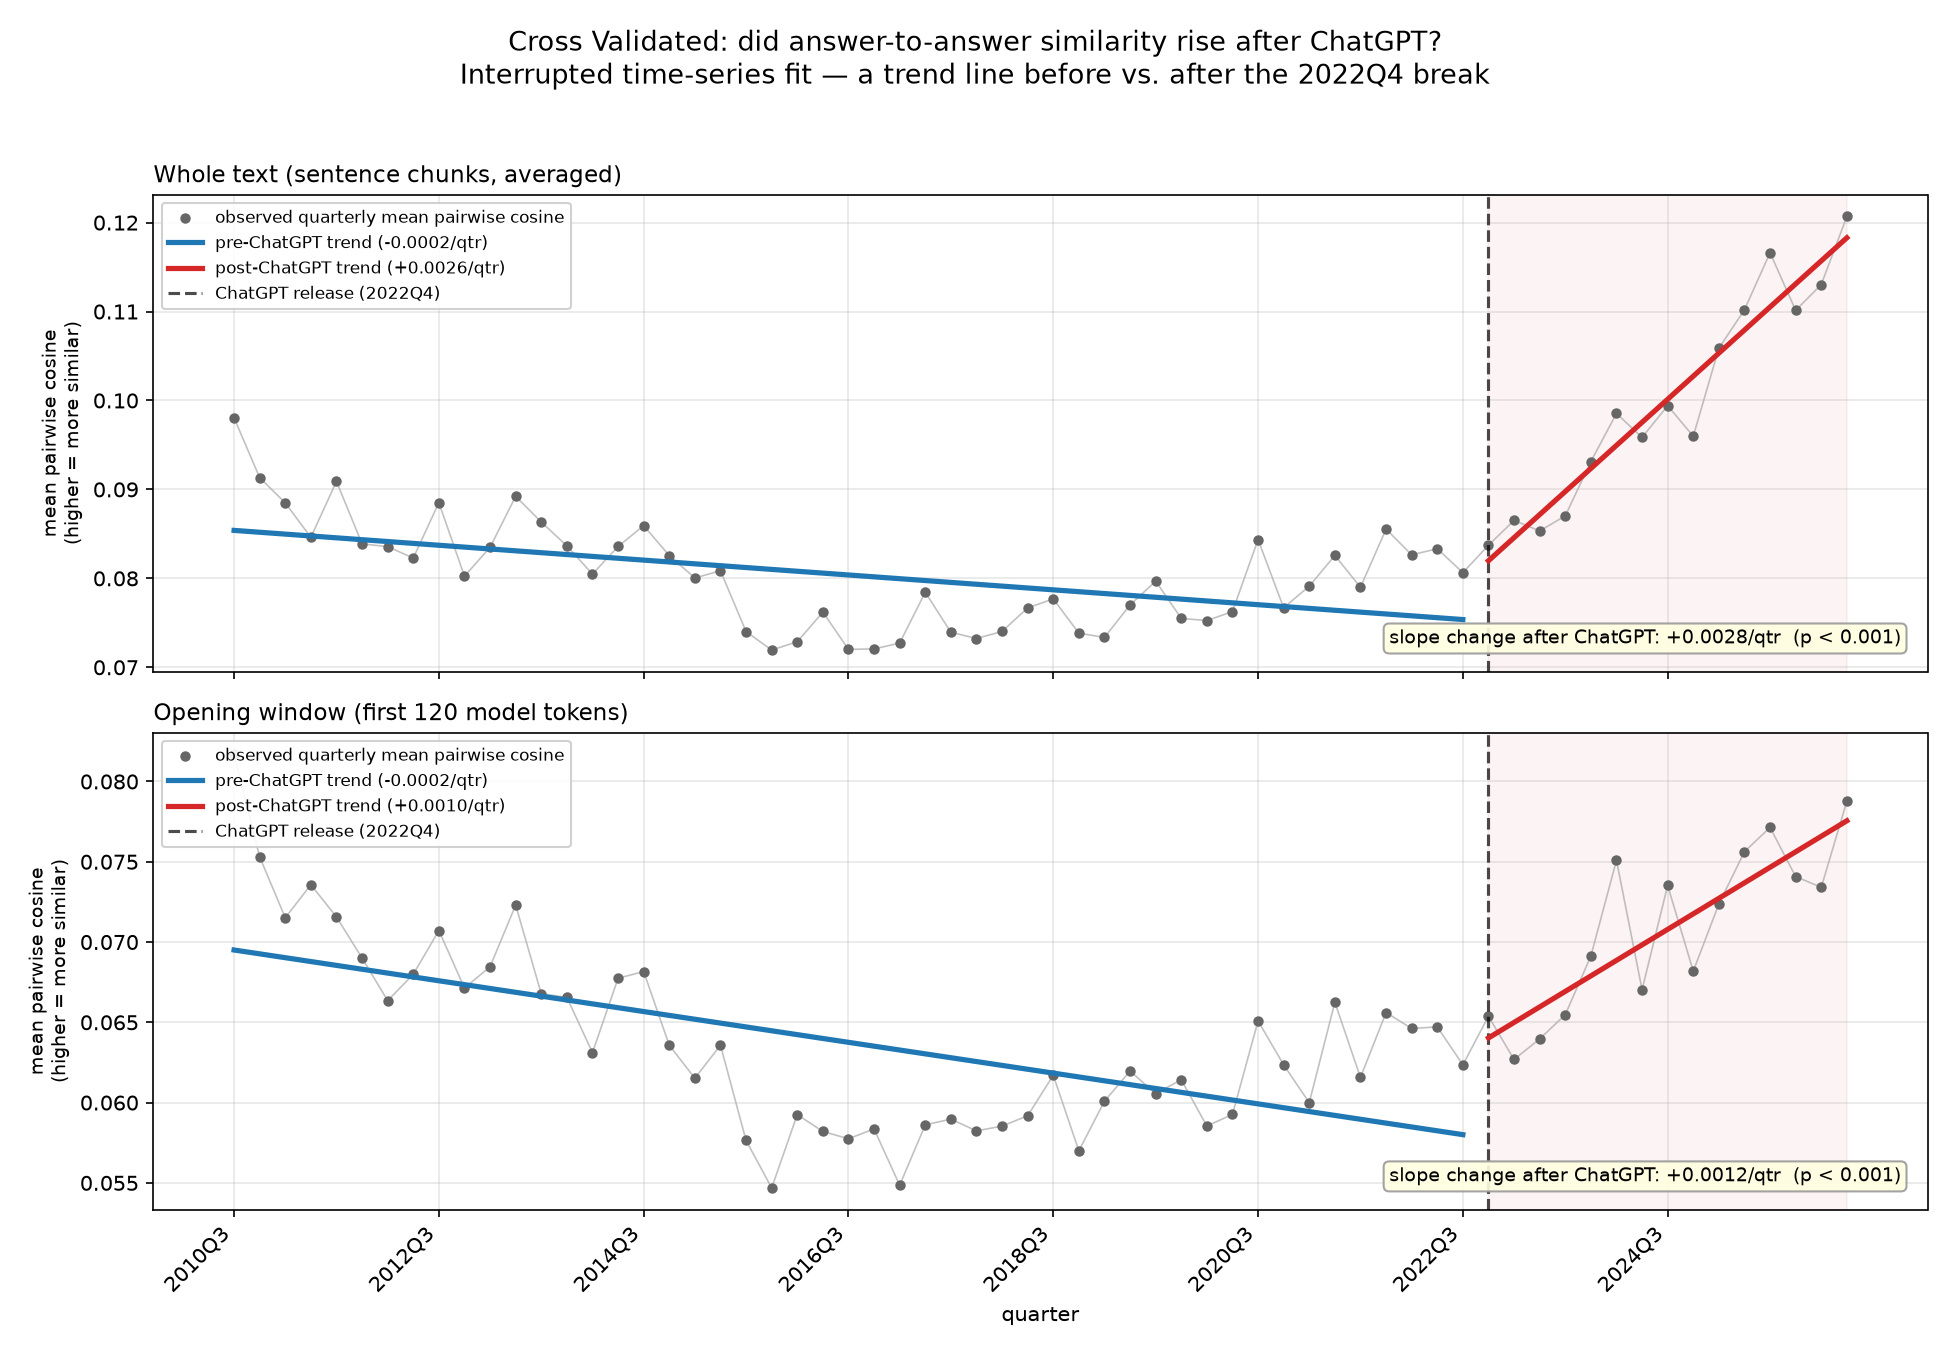
\includegraphics[width=0.75\linewidth]{fig_its_cv.png}
  \caption{How the slope change is measured, for Cross Validated. Dots: average similarity between
  answers in each quarter. Blue line: trend before ChatGPT ($-0.0002$ per quarter); red line: trend
  after ($+0.0026$). The slope change is the difference, $+0.0028$ per quarter. Top: whole answers;
  bottom: first 120 tokens only (the length check of Section~\ref{sec:alike}).}
  \label{fig:its}
\end{figure}

\paragraph{Tests.} We call each test a \emph{family}: a measure computed per corpus and quarter,
its slope-change test, and its plots, numbered as in the accompanying code. Table~\ref{tab:tests}
maps each question to its families and the corpora they use. Earlier exploratory families are
summarised in Appendix~\ref{app:exploratory}.

\begin{table}[H]
\centering
\caption{Questions, tests, and the corpora each test uses.}
\label{tab:tests}
\small
\begin{tabularx}{\linewidth}{>{\raggedright\arraybackslash}p{2.6cm}p{1.1cm}>{\raggedright\arraybackslash}Xp{1.6cm}}
\toprule
Question & Family & Test & Corpora \\
\midrule
1. More similar? & 5, 8 & Average similarity between texts each quarter; slope change at 2022Q4 & all 30 \\
2. Where stronger? & 9 & Slope change, scaled by each site's pre-2022 variability, high vs low load & 26 SE \\
3. What changed? & 13 & Same-subject similarity, number of subjects and subject mix, with subjects = 50 embedding topics & all 30 \\
 & 14 & The same, with subjects = Stack Exchange tags & 26 SE \\
 & 11 & Similarity between answers to the same question & 26 SE \\
4. Like the model? & 12 & Similarity of each answer to gpt-4o-mini's answer to the same question & 26 SE \\
\bottomrule
\end{tabularx}
\end{table}

\paragraph{Three definitions of ``the same subject''.} Question 3 needs to know which texts are about
the same thing. We use three definitions, from broad to exact:
\begin{itemize}
  \item \textbf{Embedding topics.} All sampled texts of a corpus, across all quarters, are grouped into
  50 clusters of similar vectors (k-means). A cluster is a topic; it means the same thing in every
  quarter. Available for all 30 corpora.
  \item \textbf{Stack Exchange tags.} Every Stack Exchange question carries one to five tags chosen by
  the asker from the community's vocabulary---for example \texttt{regression} and \texttt{bayesian}
  on Cross Validated, or \texttt{visas} and \texttt{schengen} on Travel. An answer inherits its
  question's tags, and two answers are on the same subject if their questions share at least one tag.
  Tags are defined by the community, not by us or by the embeddings.
  \item \textbf{The same question.} Two answers to the same question, the narrowest possible subject.
\end{itemize}

\paragraph{Subject measures.} With subjects defined, each quarter has a \emph{subject mix}: the share
of its texts in each subject. We measure three things:
\begin{itemize}
  \item \emph{Same-subject similarity}: the average similarity over pairs of texts on the same
  subject. A rise means texts on the same subject become more alike.
  \item \emph{Number of subjects}: the effective number of subjects, $e^{H}$, where $H$ is the
  entropy of the subject mix. It reads as ``how many equally common subjects this mix is worth'':
  50 if all 50 topics are equally common, 1 if every text is on one subject.
  \item \emph{Subject-mix shift}: how different the quarter's subject mix is from the mix before
  ChatGPT (all pre-2022Q4 texts pooled), measured by the Jensen--Shannon divergence \citep{lin1991}:
  0 for the same proportions, 1 for no subject in common. A rise means people now write about
  different things, in different proportions, than they used to.
\end{itemize}
The last two depend on how many texts a quarter has, and volumes fell after 2022 on several sites, so
both are computed on random samples of 100 texts per quarter, averaged over 50 draws.

\paragraph{Model anchor.} If people increasingly write like a language model, their answer to a
question should increasingly resemble the model's answer to that same question. For up to 100
sampled answers per quarter we ask gpt-4o-mini to answer the same question (title and body) as a
Stack Exchange user would, for every year---including years before ChatGPT existed, so the model acts
as a fixed ruler. Some resemblance is expected simply because both texts are about the same subject,
so we compare each human answer with the model's answer to its own question and with the model's
answers to five \emph{other} questions sharing a tag, from the same quarter. The difference, which
we call \emph{pull}, is the part of the resemblance specific to the question. In total 154,517 model
answers were generated for 157,495 human answers.

% ---------------------------------------------------------------------------------------------
\section{Results}

\subsection{Answers became more similar to each other after ChatGPT}
\label{sec:alike}

This section asks whether answers written in the same quarter resemble \emph{each other} more than
they used to (comparison with the model's own answers comes in Section~\ref{sec:model}). In 24 of 26
Stack Exchange communities the slope of answer-to-answer similarity increases after 2022Q4; the
increase is significant in 15 (all 15 survive the multiple-testing correction) and in all 4 external
corpora (Figure~\ref{fig:significance}). The typical pattern is a flat or slowly declining similarity
before ChatGPT that turns upward afterwards: 13 of the 19 significant corpora had a falling pre-2022
trend, 7 of them significantly. Two external corpora (PubMed, arXiv CS) were already rising before
2022; there the change is an acceleration rather than a reversal.

\textbf{Is it just longer answers?} Answers got longer after ChatGPT on several sites, and length
alone can raise similarity: a long answer's vector is the average of many chunk vectors, and
averaging smooths out what is specific to each chunk, pulling long answers towards a common,
generic direction---so two long answers can look similar even if they say different things. To rule
this out we repeat every test on exactly the first 120 tokens of each answer, so that all texts have
the same length (shorter answers are left out). This gives the same verdict in 26 of 30 corpora; the
four that differ (History, Astronomy, Bicycles, Photography) are significant \emph{only} in the
fixed-length version. Length does not drive the result.

\textbf{Does it depend on the encoder?} We repeated the test with a second, independently trained
encoder, BGE-small \citep{xiao2023cpack}. In the 14 high-load communities and the 4 external corpora
the two agree closely: 9 high-load communities and all 4 external corpora rise significantly with
both. In the 12 low-load communities they do not: the second encoder finds a significant rise in only
2 and a significant fall in 3 (Seasoned Advice, Bicycles, Home Improvement). The rise is therefore
robust in expert and academic writing, and encoder-dependent in everyday communities.

\begin{figure}[H]
  \centering
  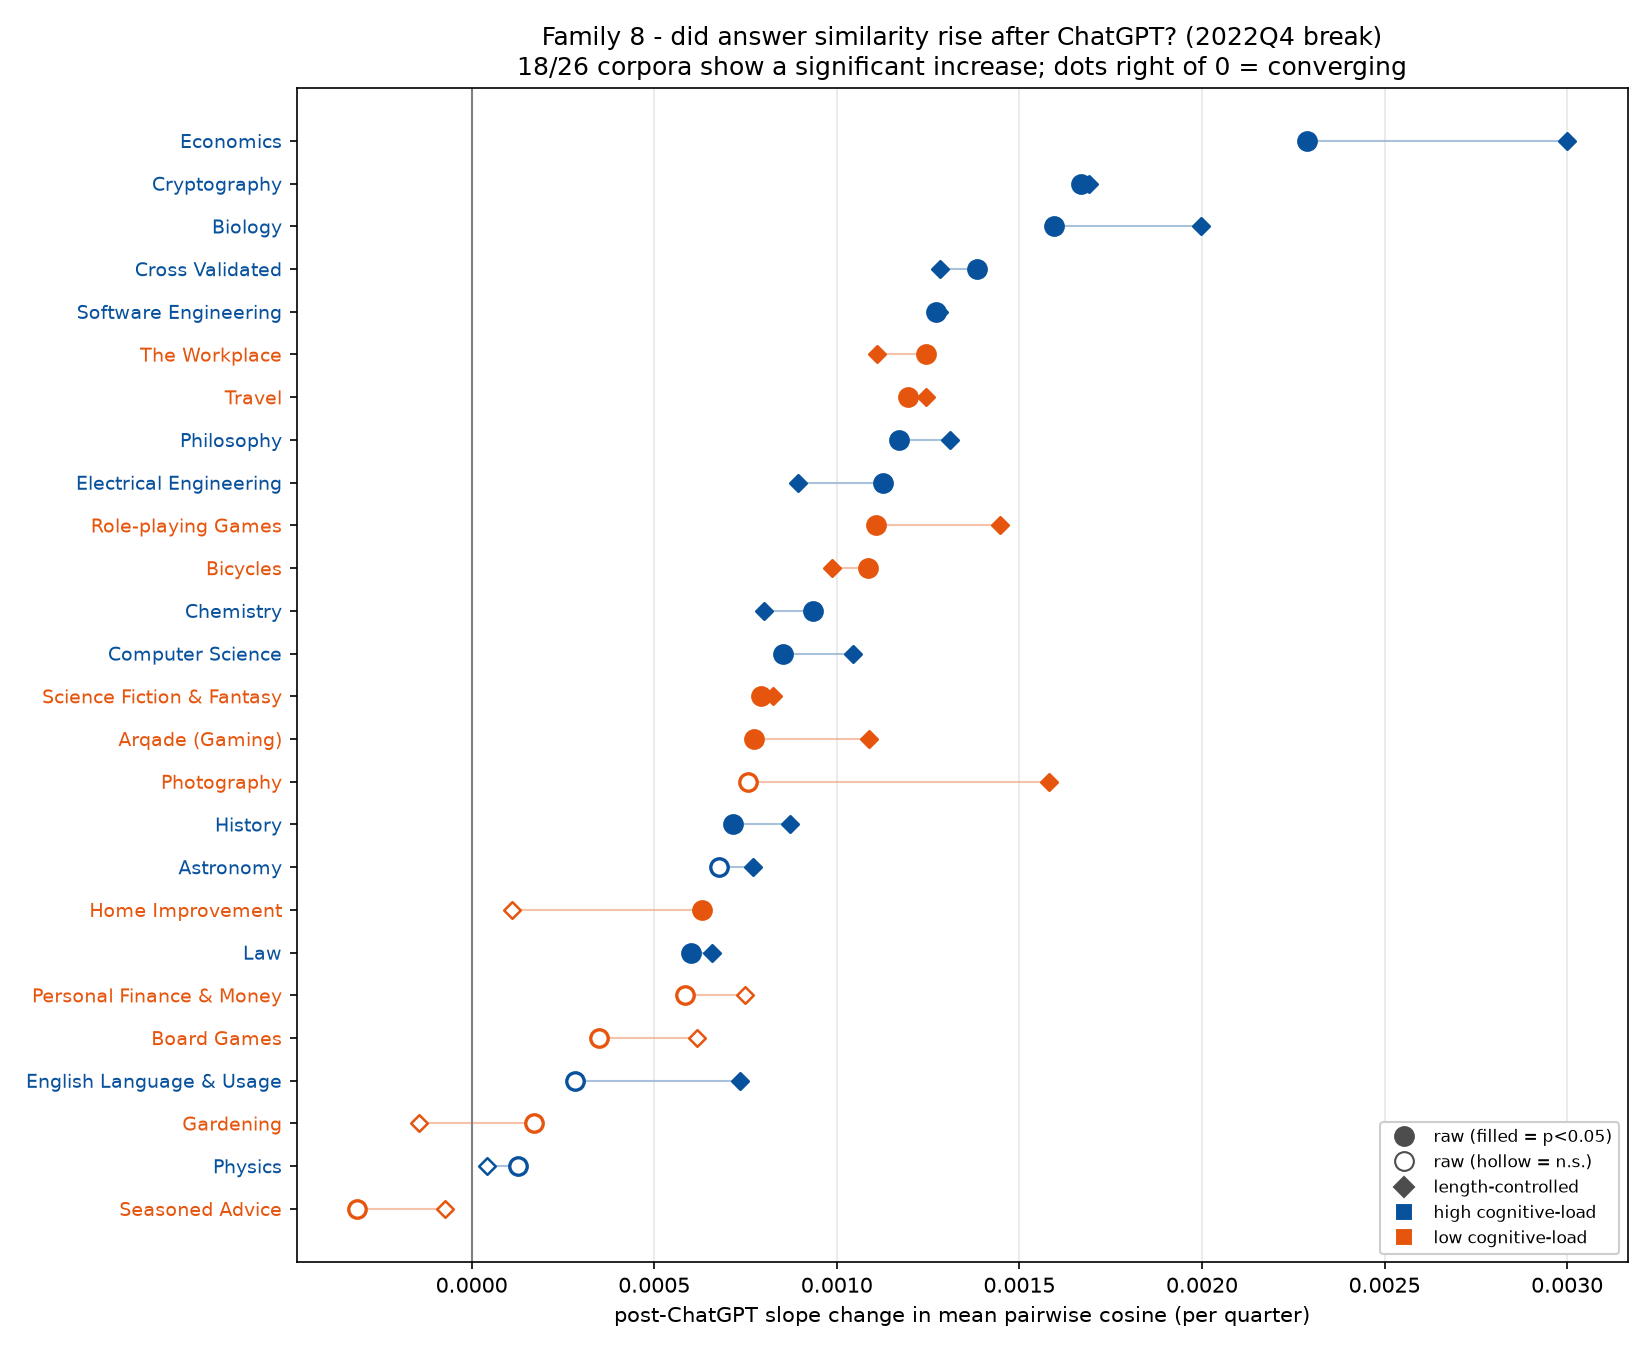
\includegraphics[width=0.8\linewidth]{fig_significance.png}
  \caption{Slope change in answer-to-answer similarity after ChatGPT, per corpus. Circles: whole
  answers (filled $=p<0.05$); diamonds: first 120 tokens only. Blue: high-load Stack Exchange;
  orange: low-load; green: external.}
  \label{fig:significance}
\end{figure}

\subsection{The turn is stronger where AI saves more effort}
\label{sec:where}

High-cognitive-load communities turn up more than low-load ones (Figure~\ref{fig:cogload}): the
change is significant in 11 of 14 versus 4 of 12 (Fisher exact $p=0.026$), and the median slope
change, scaled by each site's pre-2022 variability, is 0.20 versus 0.09 (Mann--Whitney $p=0.010$;
permutation $p=0.010$). High-load answers are somewhat longer, but answer length does not predict a
site's slope change, and the difference holds with length as a control ($p=0.026$). On the first 120
tokens alone more high-load sites are significant (13/14 vs 6/12, $p=0.021$), but the effect sizes
are closer ($p=0.06$). With the second encoder the difference is larger: 9 of 14 versus 2 of 12
significant (Fisher $p=0.019$), median scaled slope change 0.11 versus $-0.02$ (Mann--Whitney
$p=0.002$).

\begin{figure}[H]
  \centering
  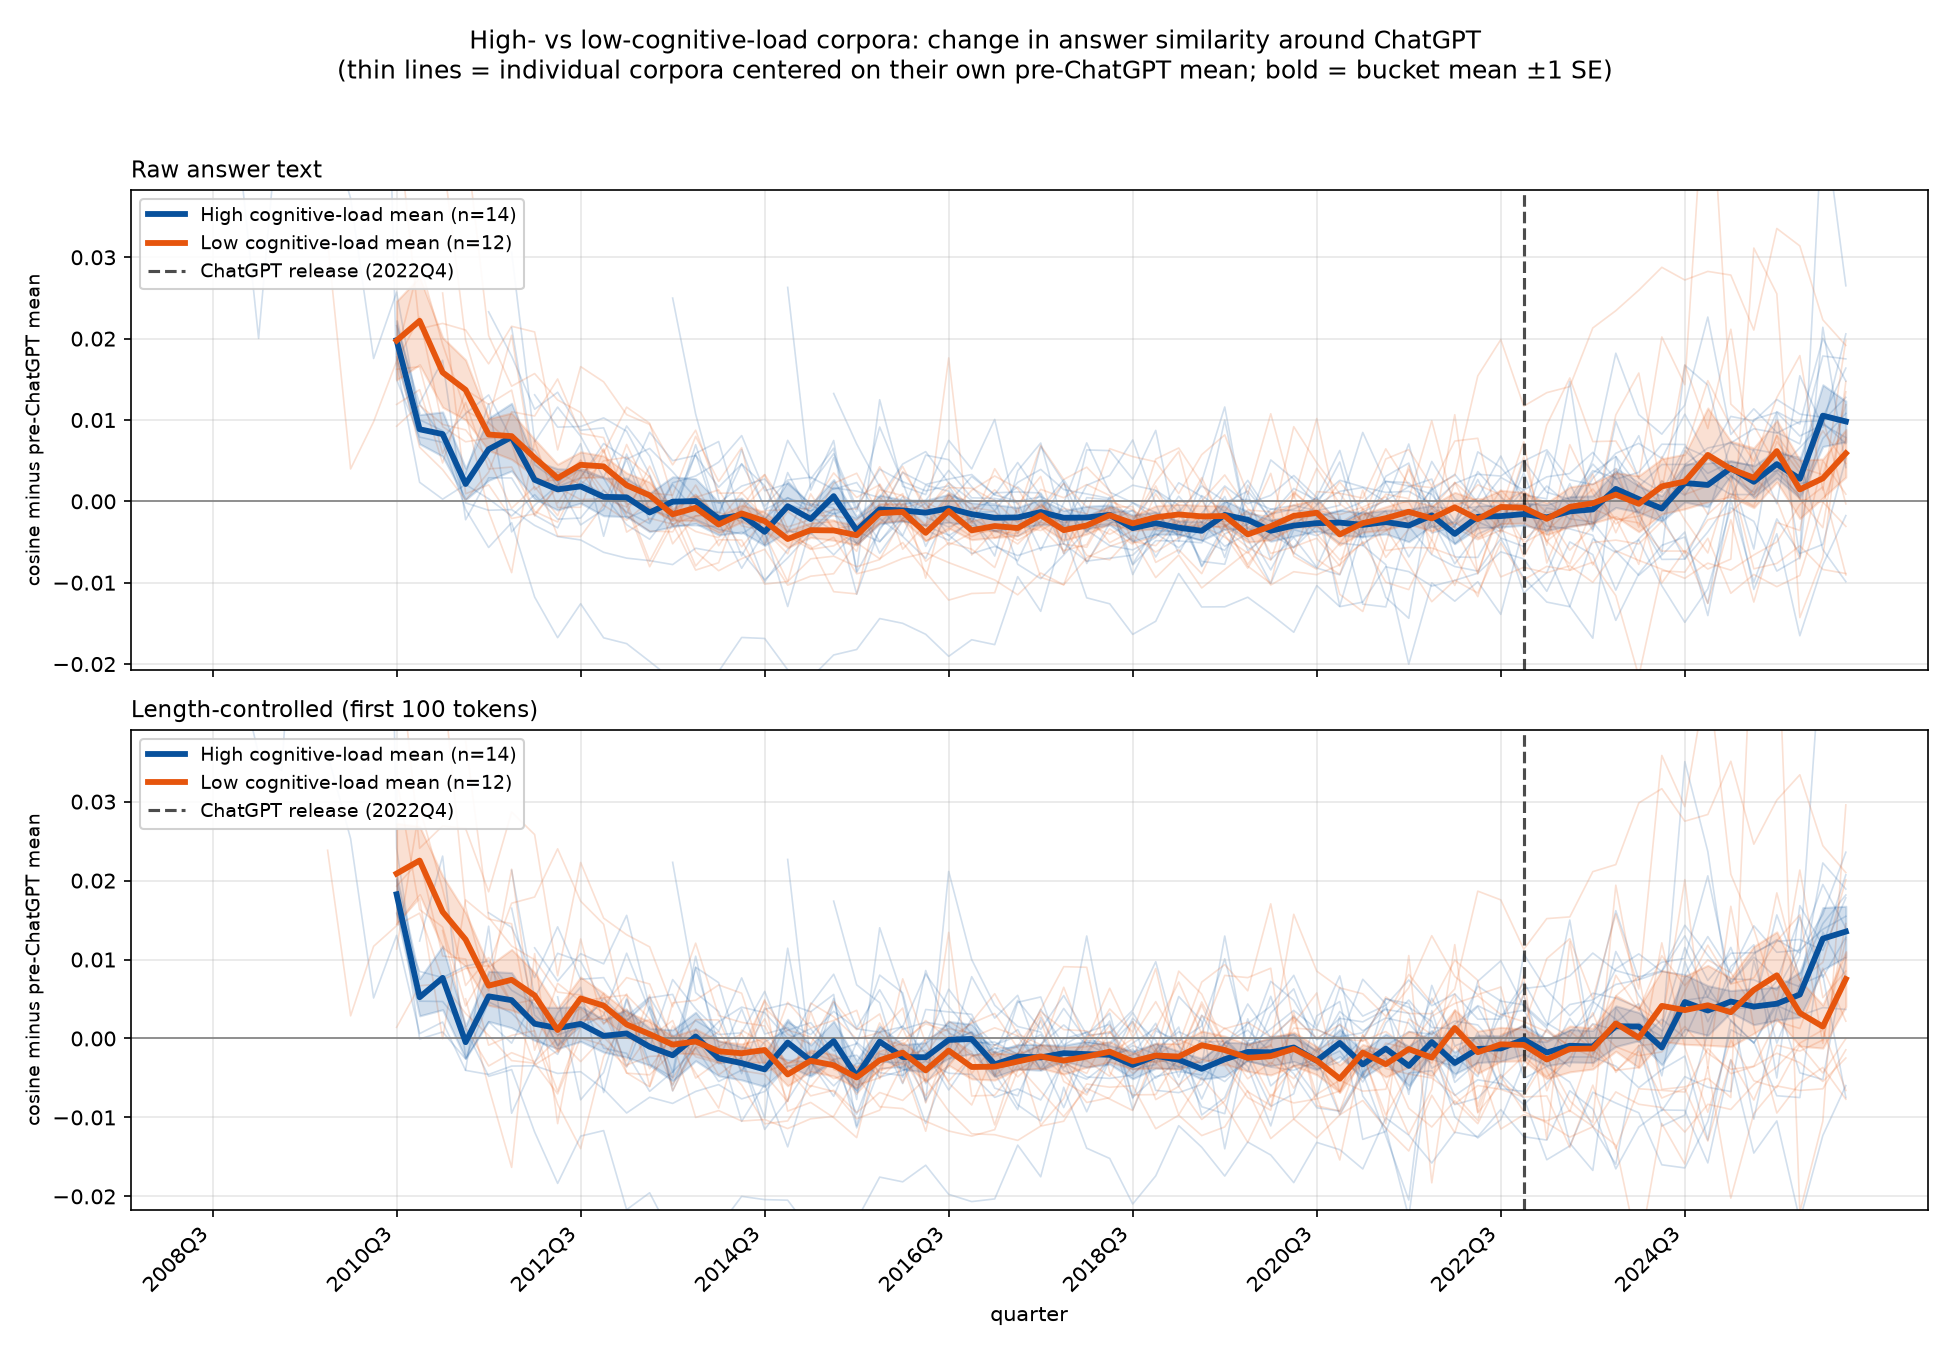
\includegraphics[width=0.62\linewidth]{fig_cogload.png}
  \caption{Slope change per Stack Exchange site, in units of its pre-ChatGPT variability; filled =
  significant. External corpora shown for reference, not part of the test.}
  \label{fig:cogload}
\end{figure}

\subsection{What changed: the subjects and the questions, more than the answers}
\label{sec:what}

Answers can become more similar for three different reasons: people write about a narrower or
different set of subjects; answers on the same subject converge; or answers to the same question
converge. Table~\ref{tab:what} tests each, using the three definitions of ``the same subject'' from
the Method section.

\begin{table}[H]
\centering
\caption{Number of corpora with a significant change after ChatGPT ($p<0.05$).}
\label{tab:what}
\small
\begin{tabularx}{\linewidth}{>{\raggedright\arraybackslash}Xcccc}
\toprule
Same subject defined as\ldots & Out of & \shortstack{Same-subject\\texts converge} & \shortstack{Subject mix\\shifts} & \shortstack{Fewer\\subjects} \\
\midrule
Embedding topics & 30 & 16 & 25 & 27 \\
\quad high / low / external & 14 / 12 / 4 & 11 / 3 / 2 & 12 / 9 / 4 & 13 / 10 / 4 \\
Stack Exchange tags & 26 & 18 & 24 & 13 \\
\quad high / low load & 14 / 12 & 9 / 9 & 12 / 12 & 8 / 5 \\
The same question & 26 & 6$^{a}$ & n/a$^{b}$ & n/a$^{b}$ \\
\quad high / low load & 14 / 12 & 4 / 2 & & \\
\bottomrule
\end{tabularx}
\par\smallskip\raggedright\footnotesize
$^{a}$ 4 remain significant after the Benjamini--Hochberg correction.
$^{b}$ Each question is asked once, so there is no mix of questions to compare across quarters.
\end{table}

\begin{figure}[H]
  \centering
  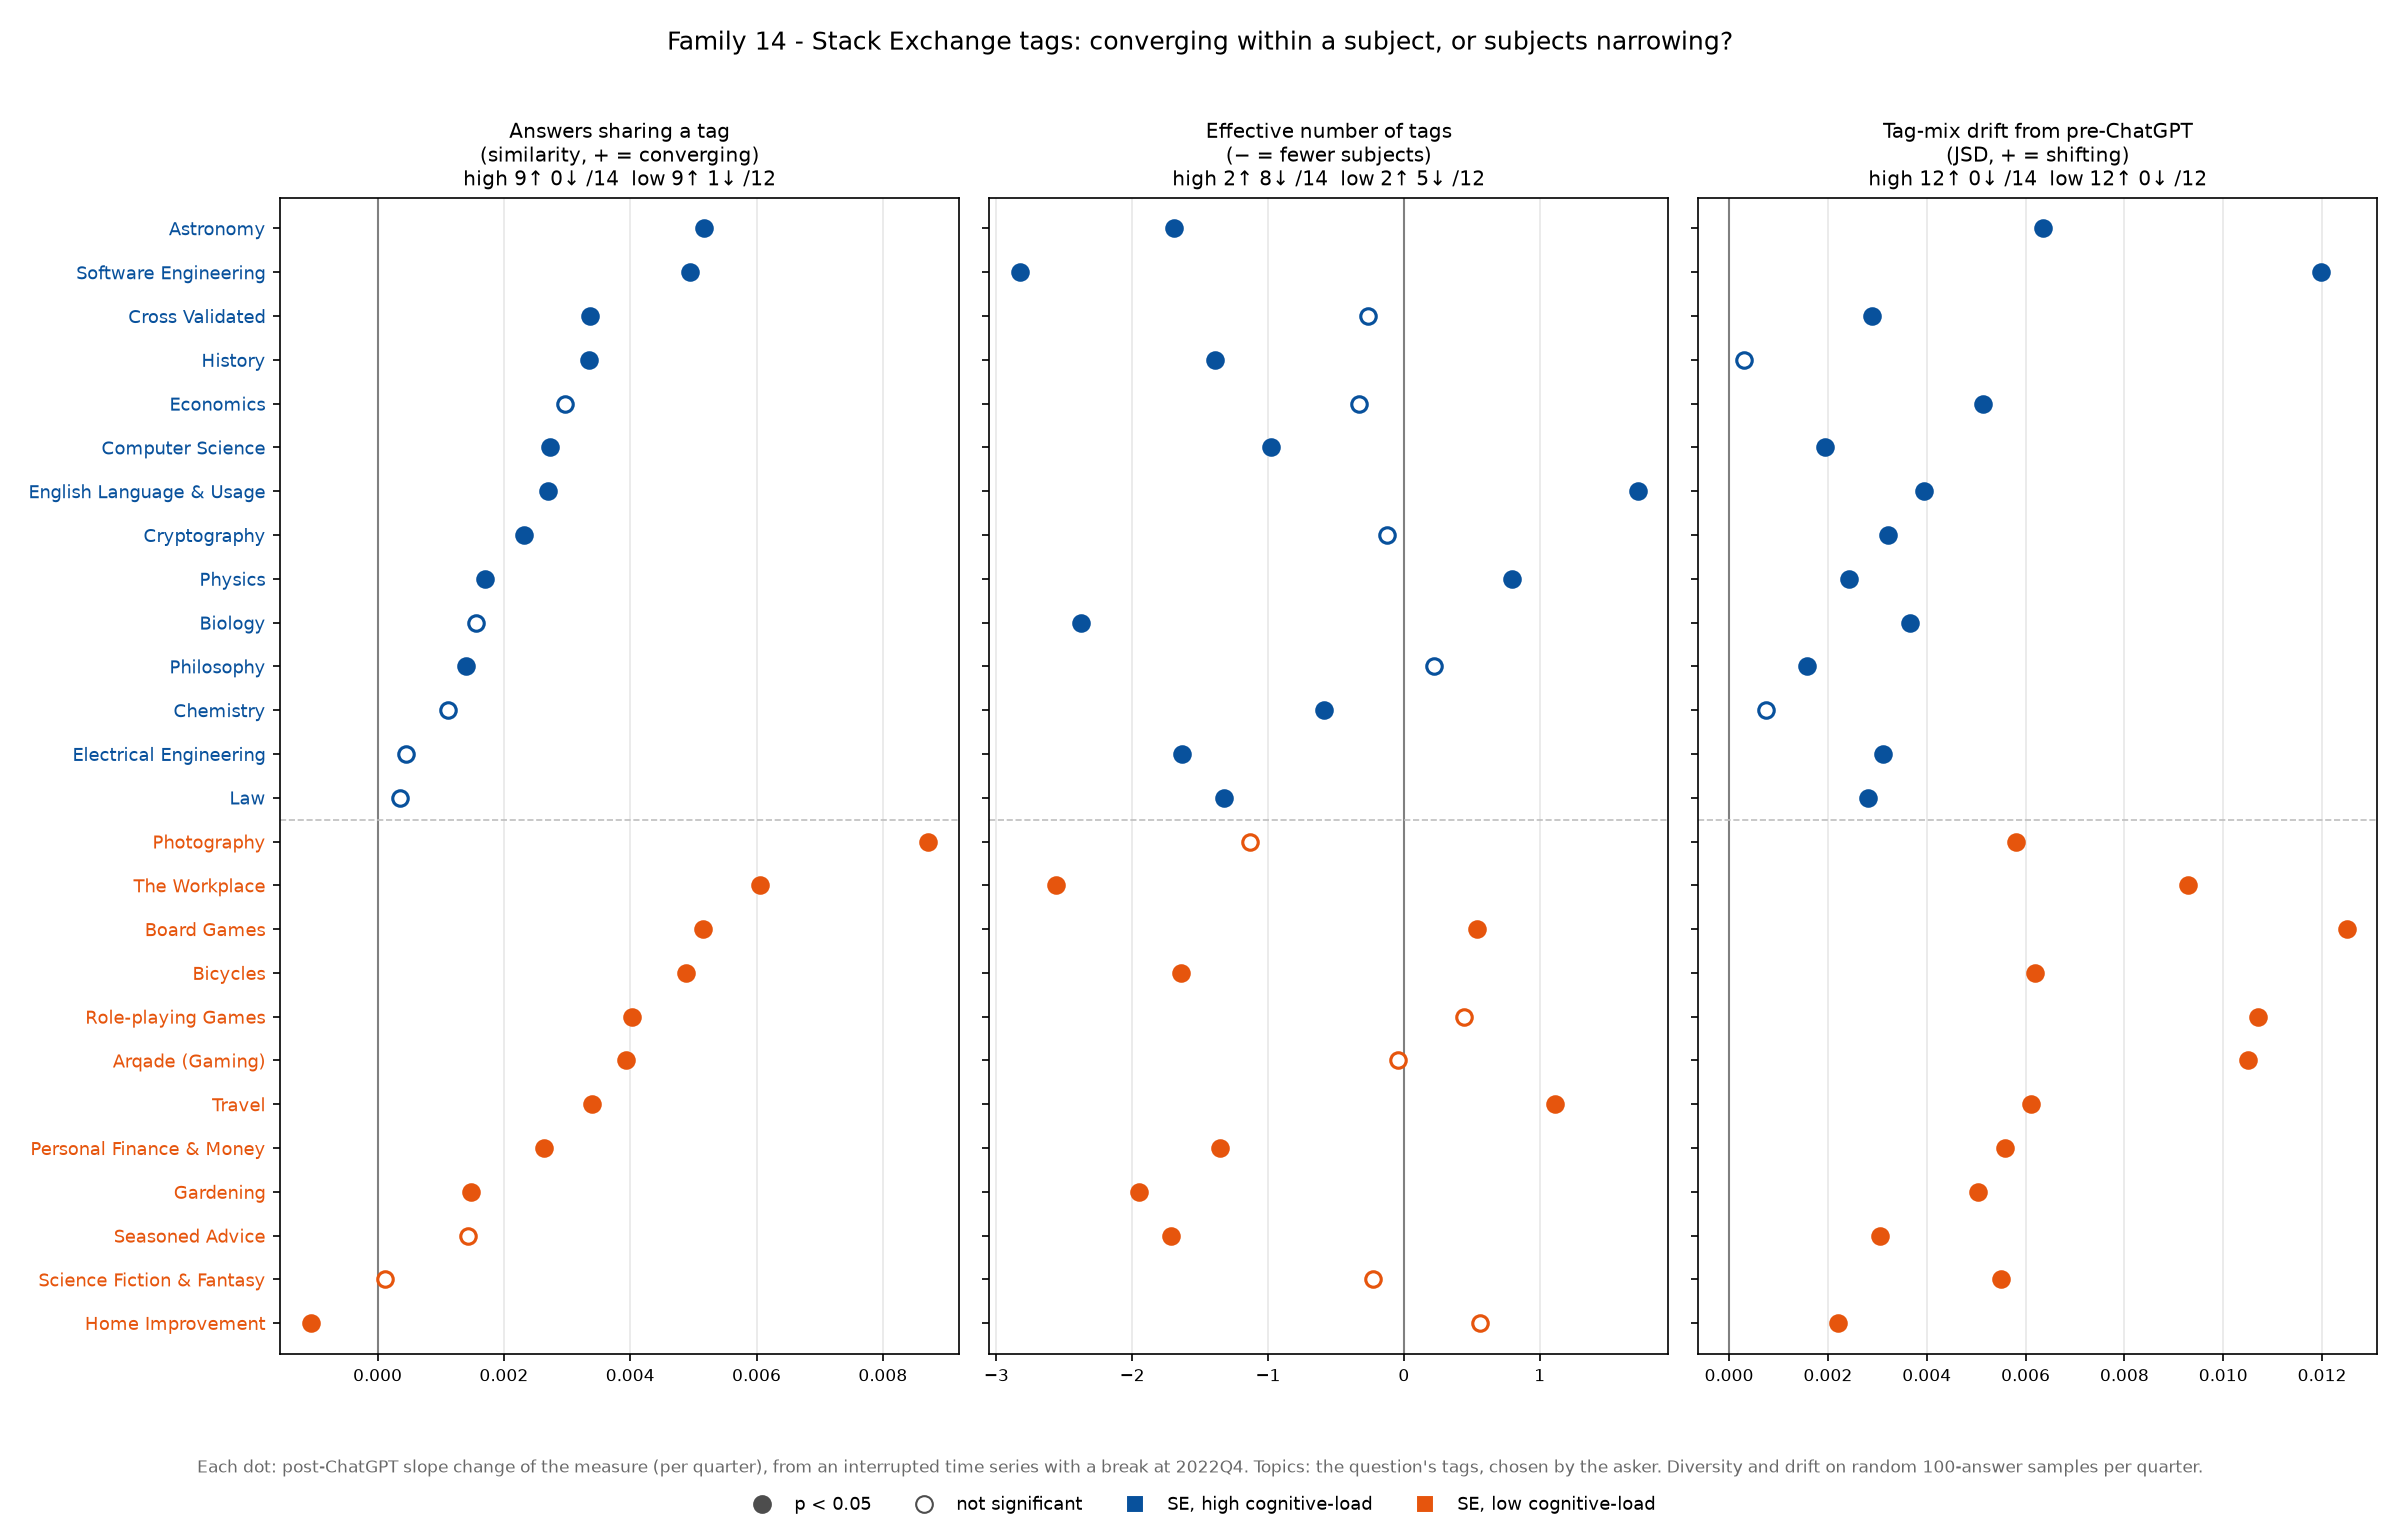
\includegraphics[width=\linewidth]{fig_tags.png}
  \caption{Subjects as Stack Exchange tags: per-site slope change in the similarity of answers
  sharing a tag (left), in the effective number of tags (centre) and in the shift of the tag mix
  from its pre-ChatGPT shape (right). Filled = $p<0.05$.}
  \label{fig:tags}
\end{figure}

Three findings follow:
\begin{itemize}
  \item \textbf{What people discuss changes almost everywhere.} The subject mix moves away from its
  pre-ChatGPT shape in 24 of 26 sites by tags and 25 of 30 corpora by embedding topics, and the number
  of distinct subjects falls in most (Figure~\ref{fig:tags}).
  \item \textbf{Answers on the same subject become more similar} in about two thirds of the sites by
  tags.
  \item \textbf{Answers to the exact same question mostly do not.} Only 6 of 26 sites show
  convergence, while any two answers from the same quarter, whatever their question, become more
  similar in 18 (Figure~\ref{fig:samequestion}).
\end{itemize}

Read together: when the question is held fixed, people answer it no more alike than before. The
convergence appears when the subject is broad, which means the \emph{questions} within a subject have
themselves become more similar---narrower, more standard, or concentrated on fewer issues. The change
is in what is asked and discussed, more than in how people answer.

Two cautions. Embedding topics are found in the same vector space in which similarity is measured,
so they can mistake answers that converge in wording for ``fewer topics''. Tags, chosen by askers, do
not have this problem; that is why the two definitions disagree on low-load sites (3 versus 9
converging), and why we rely mainly on tags. And the number of distinct subjects falls on only half
the sites by tags; on four it rises.

\begin{figure}[H]
  \centering
  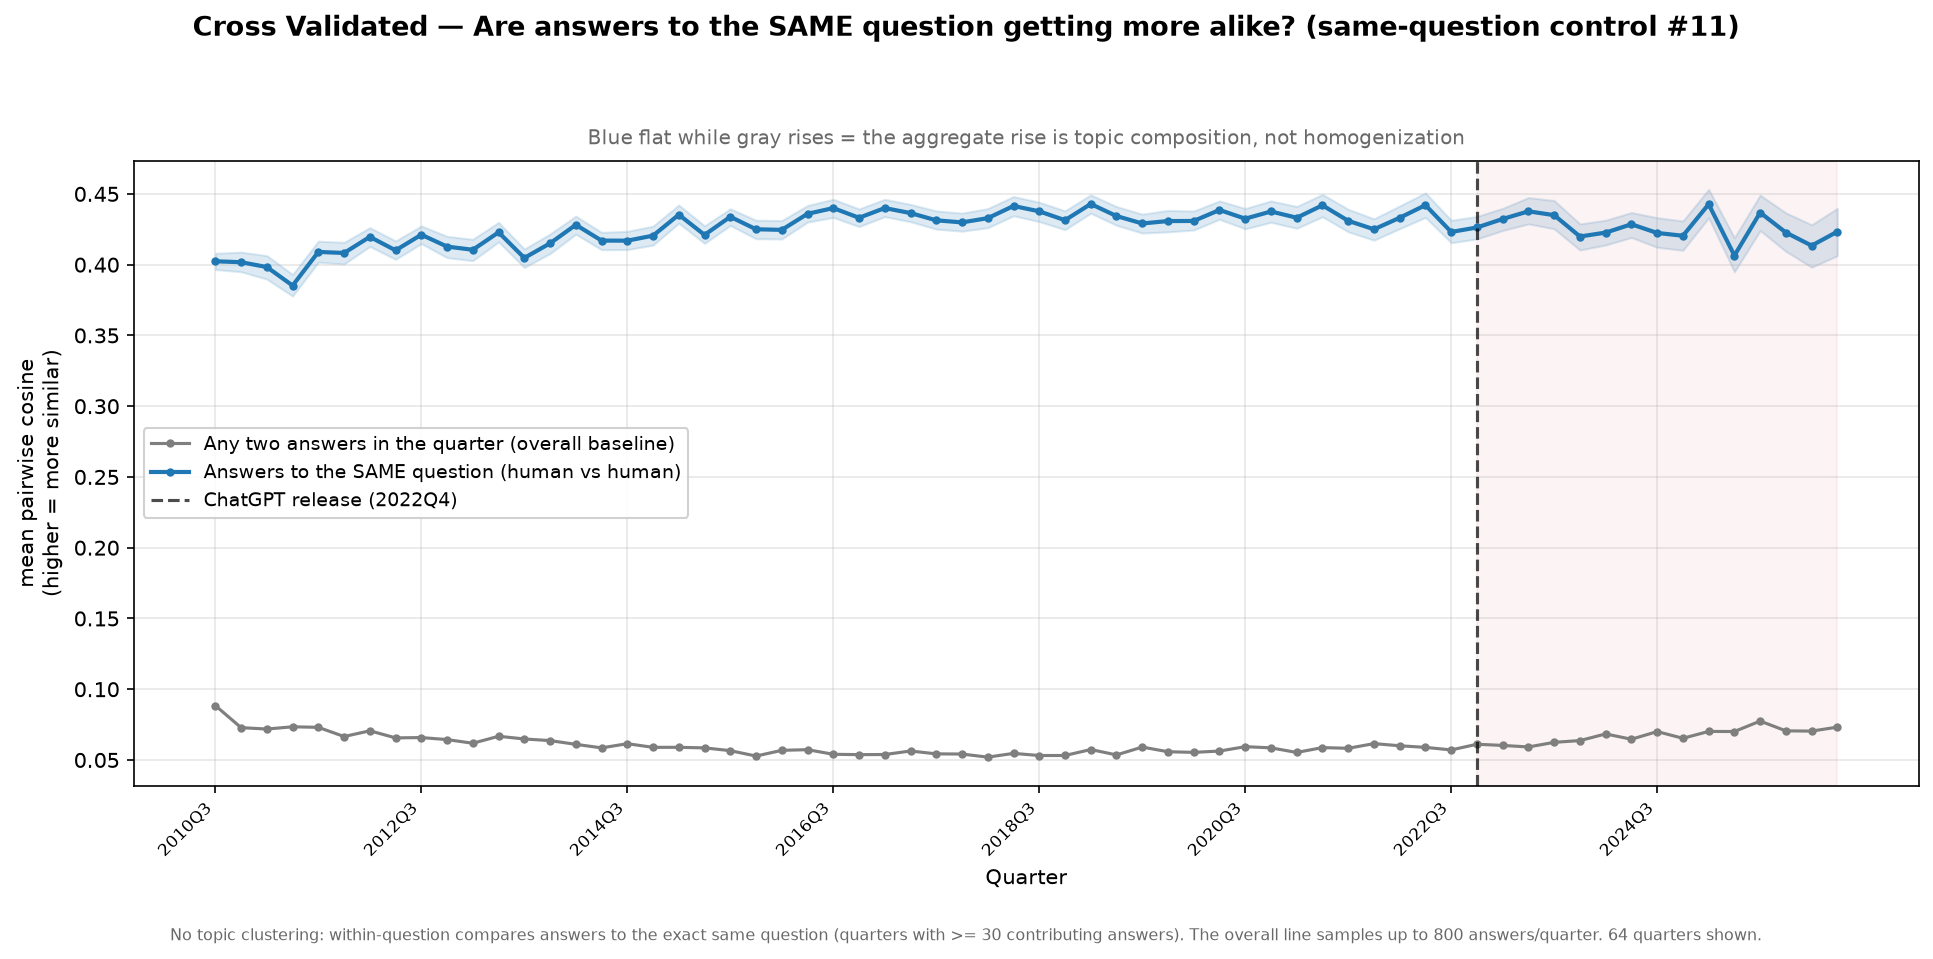
\includegraphics[width=0.85\linewidth]{fig_same_question.png}
  \caption{Left: similarity between answers to the same question. Right, for reference: similarity
  between random pairs of answers from the same quarter, whatever their question. Filled = $p<0.05$.}
  \label{fig:samequestion}
\end{figure}

\subsection{People do not write more like the model}
\label{sec:model}

If people increasingly wrote like a language model, a human answer should increasingly resemble the
model's answer to the same question---and more so than it resembles the model's answers to other
questions on the same subject, which only reflect the shared subject. The test is sensitive: a human
answer is much closer to the model's answer to its own question than to the model's answers to other
same-tag questions (median similarity 0.64 versus 0.23). But that closeness does not grow after
ChatGPT (Figure~\ref{fig:anchor}):
\begin{itemize}
  \item similarity to the model's answer to the same question rises in 8 of 26 sites and falls in 2
  (on the first 120 tokens: rises in 5, falls in 3);
  \item the question-specific part (\emph{pull}) rises in 2 and falls in 6, none surviving the
  multiple-testing correction.
\end{itemize}
People's answers have not moved towards what the model says. The model's answers are stable: three
independent answers to the same question have an average similarity of 0.92.

\begin{figure}[H]
  \centering
  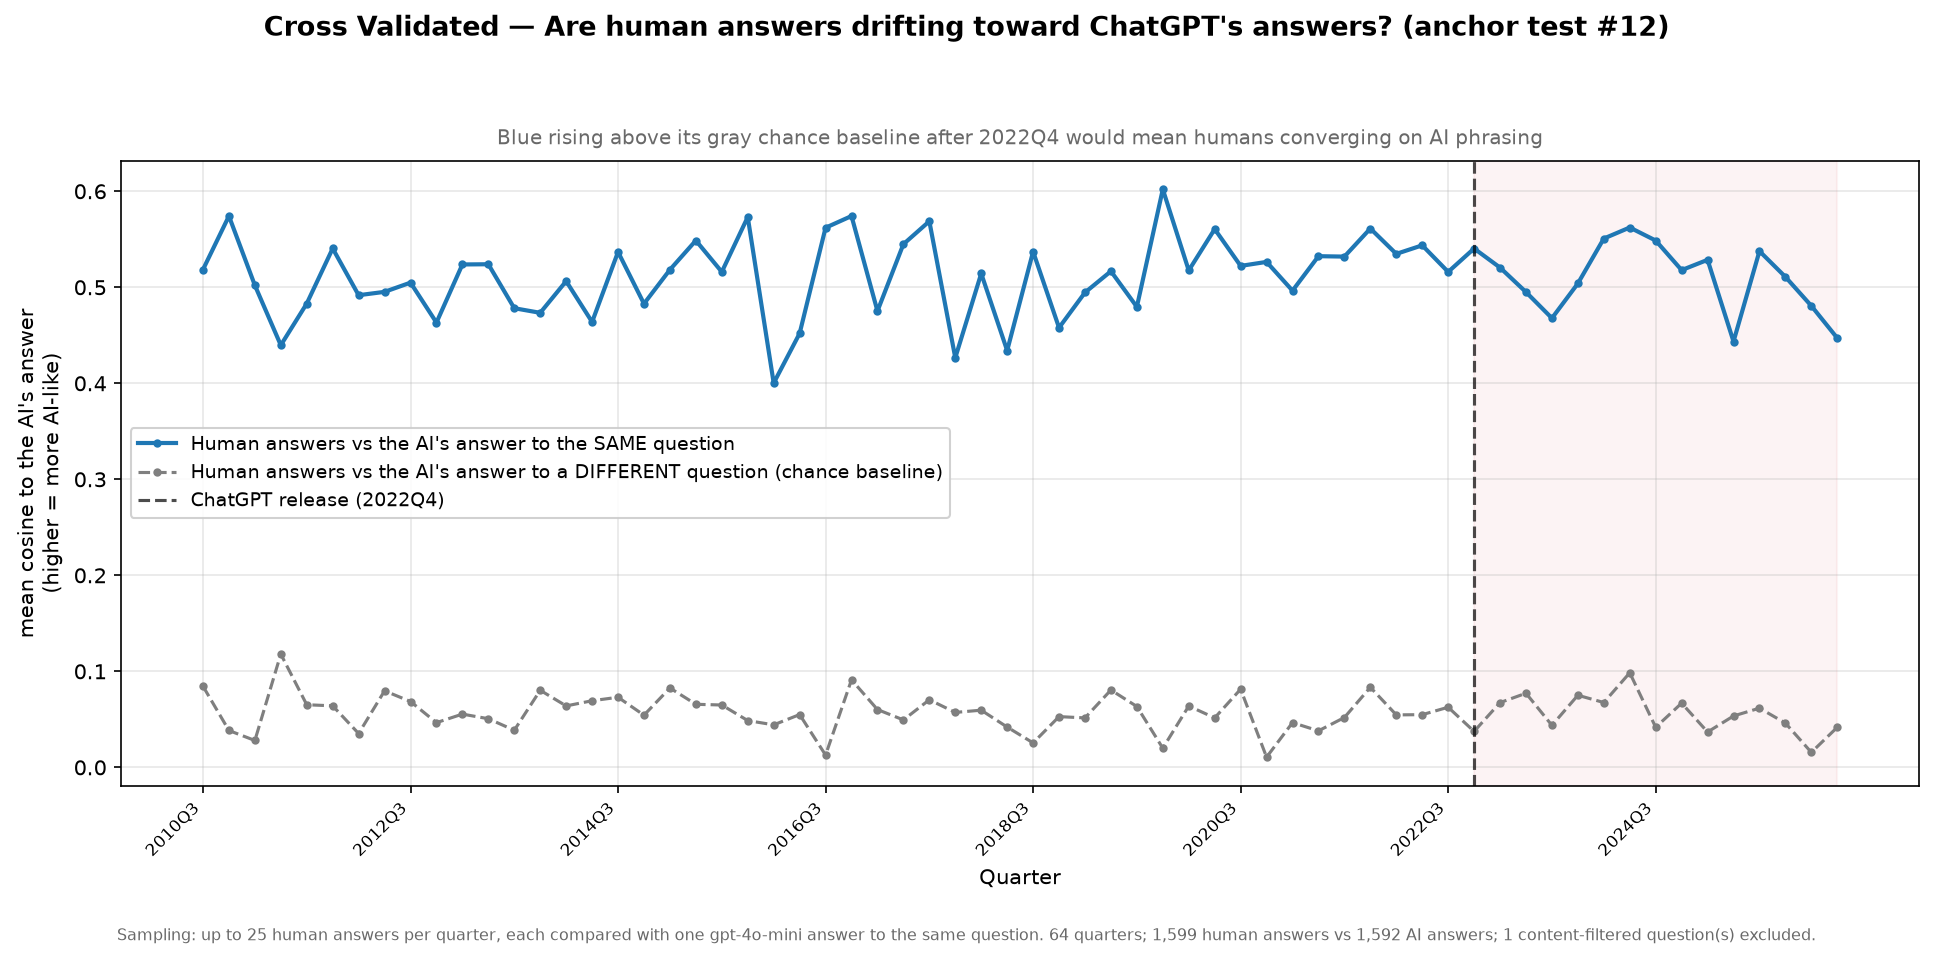
\includegraphics[width=\linewidth]{fig_anchor.png}
  \caption{Per-site slope change in similarity to gpt-4o-mini's answer to the same question (whole
  text and first 120 tokens) and in pull (same question minus same-tag questions). Filled = $p<0.05$.}
  \label{fig:anchor}
\end{figure}

\subsection{Robustness}

\begin{table}[H]
\centering
\caption{Robustness checks.}
\label{tab:robust}
\small
\begin{tabularx}{\linewidth}{p{4.2cm}X}
\toprule
Check & Result \\
\midrule
Answer length & First 120 tokens only: same verdict in 26/30 corpora; the 4 differences are significant only at fixed length. Only each text's first $K$ chunks (Cross Validated $K=3$, PubMed $K=4$): still significant. \\
Second encoder & BGE-small \citep{xiao2023cpack} on all 30 corpora: same verdict in 21/30 (whole text) and 20/30 (first 120 tokens); quarterly series correlate at a median of 0.66. High load: 11/14 agree (9 significant with both). External: 4/4. Low load: 6/12 agree; BGE finds 2 significant rises and 3 significant falls. High vs low (family 9): 9/14 vs 2/12, $p=0.019$. \\
Number of topics & 25 and 100 instead of 50 topics: the same conclusions (within-topic convergence 9--12/14 high vs 3--5/12 low; diversity falls in 24--26/30). \\
Sample size & Topic diversity and drift on fixed 100-text samples, as volumes fell after 2022: conclusions unchanged. \\
Model answers & One versus three answers per question (Economics): mean similarity between answers 0.92, so one is enough. \\
\bottomrule
\end{tabularx}
\end{table}

% ---------------------------------------------------------------------------------------------
\section{Discussion}

The pattern is consistent across tests. Online answers became more similar to one another after
ChatGPT---robustly in expert and academic communities, less clearly in everyday ones---mainly because
the questions people bring and the subjects they discuss narrowed and shifted. People answering the same question do not converge, and they do not converge on the
model's own answers.

One plausible mechanism is substitution: routine, well-defined questions that a chatbot can answer
privately no longer reach public forums, which shifts and narrows what remains---especially in
expert communities, where a model saves the most effort. That would explain why the subject mix moves
almost everywhere, why same-subject answers converge, and why same-question answers do not. Our data
are consistent with this reading but do not prove it.

This form of homogenization matters. A shrinking, shifting set of public questions is a narrowing of
the public conversation itself: the long tail of unusual questions, and the record of how people
reasoned about them, is what search engines, students and future models draw on. Because the change
is measurable, it can be monitored. We maintain an open tracker that weekly collects Google's top
results for 45 informational questions in five domains, fetches the full pages, and measures how much
they repeat one another \citep{friedman2023vendi}; it began in October 2026 and will need several
months before trends can be read.

\begin{framing}
How strong a claim should this section make? From most to least cautious: (a) ``a specific, measurable
narrowing worth monitoring''; (b) ``an early-warning sign of a narrowing public conversation'';
(c) ``evidence that AI is reshaping what people ask in public''.
\end{framing}

% ---------------------------------------------------------------------------------------------
\section{Limitations}

\begin{itemize}
  \item \textbf{Timing is not causation.} The break is fixed at ChatGPT's release; other changes
  happened in the same period (falling Stack Exchange volumes, platform policies, the pandemic, which
  is visible as a 2020 jump in Travel).
  \item \textbf{Small effects.} Slope changes are on the order of $10^{-3}$ per quarter; with many
  quarters, small effects become significant. They accumulate to a meaningful share of the
  between-quarter variation, but they are not large.
  \item \textbf{Encoder dependence in everyday communities.} The main results use one encoder. A
  second agrees in expert and academic corpora, but in low-load communities the rise depends on the
  encoder (Section~\ref{sec:alike}); claims about everyday writing are therefore weaker.
  \item \textbf{Our own labels.} The high/low cognitive-load split is our classification of each
  community; the 26 sites are a small sample for a group comparison.
  \item \textbf{Low load is Stack Exchange only.} All external corpora are high-load.
  \item \textbf{The model anchor is a proxy.} gpt-4o-mini stands in for the different chatbots people
  actually used between 2022 and 2026.
  \item \textbf{Many tests.} We report counts after multiple-testing correction where it matters, and
  report results that do not support our reading (e.g.\ low-load embedding topics, model anchor).
\end{itemize}

% ---------------------------------------------------------------------------------------------
\section{Conclusion}

Generative AI did not make everyone write the same way, and people do not write like the model. But
online answers did become more similar to one another after ChatGPT---clearly in expert and
academic communities, less clearly in everyday ones---because what people ask and discuss in public
narrowed and shifted. That is a specific, measurable form of
homogenization, and one worth watching.

\appendix
\section{Exploratory analyses}
\label{app:exploratory}

Before the main analysis we ran several simpler measures. They are kept in the code and results
(folder \texttt{artifacts/\allowbreak exploratory}) but superseded:

\begin{table}[H]
\centering
\small
\begin{tabularx}{\linewidth}{lp{3.2cm}X}
\toprule
Family & Measure & Finding and why superseded \\
\midrule
1 & Lexical diversity and surface features & Rises after ChatGPT only because answers got longer; flat at fixed length \citep{mccarthy2010}. \\
2 & Length-window sweep & Confirms family 1 at 50--200-token windows. \\
3 & LSA (bag-of-words) similarity & Length artifact like family 1; replaced by sentence embeddings. \\
4 & LDA topics & Topic mix nearly unchanged; replaced by embedding and tag topics. \\
6 & BERTopic topics & Leaves about half of the texts unassigned, so within-topic results describe a selected half; replaced by families 13 and 14, kept for topic labels \citep{grootendorst2022}. \\
7 & High- vs low-score answers & Both tiers rise (two sites); the rise is not confined to low-quality answers. \\
\bottomrule
\end{tabularx}
\end{table}

\bibliographystyle{plainnat}
\bibliography{references}

\end{document}
